\section{Datensatz}
\label{Datensatz}

Die verwendeten Daten stammen aus dem \textit{KIT Energy Smart Home Lab (ESHL)}. Das ESHL ist ein $60 m^2$ Apartment mit intelligenten Haushaltsger"aten und soll einen m"oglichen zuk"unftigen Haushalt simulieren. Die Daten des ESHL wurden "uber fast 3 Jahre zwischen dem 22.08.2011 und dem 31.07.2014 aufgezeichnet, weisen aber einige L"ucken auf. F"ur die Messungen wurden mehrere Smart Meter verwendet, bei Gro{\ss}verbrauchern wie etwa dem Boiler wurden dabei alle drei Phasen gemessen, sie sind durch die Nummer des Smart Meters in den Daten identifizierbar. Bei den restlichen Ger"aten wurde nur je eine Phase gemessen, das hei{\ss}t, dass je 3 Ger"ate an einem Smart Meter angeschlossen sind. Sie sind durch die Nummer des Smart Meters in Kombination mit Nummer des verwendeten Ports identifizierbar. Wie viele Phasen zur Messung eines Ger"ats verwendet wurden l"asst sich dem Controller entnehmen.
\begin{table}[h]
\begin{tabular}{l|l|l|l|l|l}
UUID & Name & Klassifikation & Controller & Meter & Port \\
\hline
...-5602c0a80114 & DRYER & APPLIANCE & 1 & 3 & 0 \\
...-5604c0a80114 & WASHINGMACHINE & APPLIANCE & 1 & 7 & 2
\end{tabular}
\caption["Ubersicht Ger"atezuordnung]{Beispiele f"ur Ger"atezuordnung, die Waschmaschine ist an (Smart-)Meter 7 Port 2 angeschlossen.}
\label{profile01458}
\end{table}



\subsection{Gemessene Daten}
\label{Gemessene Daten}

Die Daten des \textit{KIT Energy Smart Home Lab} besitzen folgendes Format. \\
\begin{table}[h]
\begin{tabular}{l|l|p{1cm}|p{1cm}|p{1cm}|p{1cm}|p{1cm}|p{1.2cm}|p{2cm}}
Unixtime & UUID & Con-troller & Meter & Port & Span-nung & Strom-st"arke & Wirk-leistung & Wirkl. \newline aggregiert \\
\hline
1382291846 & ...-5604c0a80114 & 1 & 7 & 2 & 218.5 & 8.96 & 1956 & 145550  \\
1315269463 & ...-5602c0a80114 & 1 & 3 & 0 & 223.8 & 13.16 & 2950 & 38300 \\
1315269465 & ...-5602c0a80114 & 1 & 3 & 0 & 223.9 & 12.5 & 2796 & 38300
\end{tabular}
\caption[Format ESHL Daten]{Format ESHL Datensatz.}
\label{profile01458}
\end{table}

Controller, Meter und Port werden, wie oben beschrieben, verwendet, um einen Datenpunkt einen eindeutigen Ger"at zuzuordnen. Hier ist zu beachten, sich diese Werte immer nur gemeinsam verwendet werden d"urfen.
Die Spalte mit der UUID-Zuordnung wird ignoriert, denn sie enth"alt ebenfalls die Information um welches Ger"at es sich handelt und ist somit Redundant zu Controller, Meter und Port. \\
Ein Datenpunkt enth"alt die gemessene Spannung, die Stromst"arke und die Wirkleistung. Es wird zus"atzlich die aggregierte Wirkleistung gemessen, welche aber zun"achst ignoriert wird, da sie sich aus der Wirkleistung berechnen l"asst. \\
Eine Besonderheit stellt das Aufzeichnungsintervall dar. Die Smart Meter erzeugen jede Sekunde einen neuen Datenpunkt f"ur jeden Port, dieser wird aber nur gespeichert, wenn sich die Wirkleistung im Vergleich zum letzten gespeicherten Punkt um 5 Watt Wirkleistung unterscheidet. So werden insbesondere lange \textit{Off} Phasen auf einen Datenpunkt komprimiert, es gehen aber auch kleinere Schwankungen in der Wirkleistung von sehr verbrauchsarmen Ger"aten verloren.


\subsection{Berechnete Daten}
\label{Berechnete Daten}

Die Messung von Spannung und Stromst"arke erlaubt es eine Vielzahl von Energiewerten zu berechnen, in diesem Abschnitt werden die Schein- und Blindleistung vorgestellt, das Kapitel zur Vorverarbeitung wird zus"atzlich eine Form der Normalisierung vorstellen. 
Die Scheinleistung ist das Produkt aus Spannung und Stromst"arke und ist die gesamte, aus dem Netz gezogene Leistung:\\ $Scheinleistung = Spannung * Stromst"arke$\\[0.5cm]
Zur Berechnung der Blindleistung werden Schein- und Wirkleistung genutzt, die Blindleistung ist dabei Leistung, die aus dem Netz gezogen wird ohne tats"achlich genutzt zu werden:\\ $Blindleistung = \sqrt{Scheinleistung^2 - Wirkleistung^2}$ \\


\subsection{Die Waschmaschine}
\label{Die Waschmaschine}

Die Waschmaschine ist ein besonders interessantes Ger"at f"ur die Klassifikation, denn sie hat nicht nur einen \textit{On-} und einen \textit{Off-Zustand}, sondern einen Motor, der mit verschiedenen Drehzahlen laufen kann, ein Heizelement und eine Pumpe. F"ur die Waschmaschine existieren au{\ss}erdem einige annotierte Waschg"ange die als Trainingsdaten verwendet werden k"onnen.\\
\begin{table}[h]
\begin{tabular}{l|l|l|l|l}
Profil & Startzeit (Unix) & Endzeit (Unix) & Dauer (Sekunden) & Datum \\
\hline
Profil 0 & 1382290611 & 1382296244 & 5633 & 20.10.2013 \\
Profil 1 & 1382363246 & 1382369468 & 6222 & 21.10.2013 \\
Profil 4 & 1382900551 & 1382905960 & 5409 & 27.10.2013 \\
Profil 5 & 1383173215 & 1383180425 & 7210 & 30.10.2013 \\
Profil 8 & 1384066710 & 1384072260 & 5550 & 10.11.2013
\end{tabular}
\caption["Ubersicht Trainingsdaten]{"Ubersicht "uber die annotierten Waschg"ange, die als Trainingsdaten verwendet werden.}
\label{profile01458}
\end{table}\\
Die Waschg"ange sind mit sechs verschiedenen Klassen Sigma 0 bis Sigma 5 annotiert, Sigma 0 ist der \textit{Off-Zustand}. Sigma 1 ist ein normaler Schleudervorgang, hier sind Phasen mit 200-350 Watt und dazwischen kurze Pausen mit ca. 4 Watt Verbrauch typisch.
Sigma 2 ist ein Heizvorgang, dieser kennzeichnet sich durch einen Verbrauch "uber 1700 Watt.
Sigma 3 und Sigma 4 sind Pumpvorg"ange und werden durch Verbrauchspitzen von wenigen Sekunden charakterisiert. Unterschieden werden sie anhand der H"ohe der Spitze, ein Vorgang Sigma 4 folgt immer auf einen Vorgang Sigma 3 mit einem Abstand von 50 bis 80 Sekunden.
Sigma 5 ist das Ausschleudern, es ist ebenfalls ein Schleudervorgang, der aber im Gegensatz zu Sigma 1 ohne Pausen ausgef"uhrt wird.
\begin{figure}[ht]
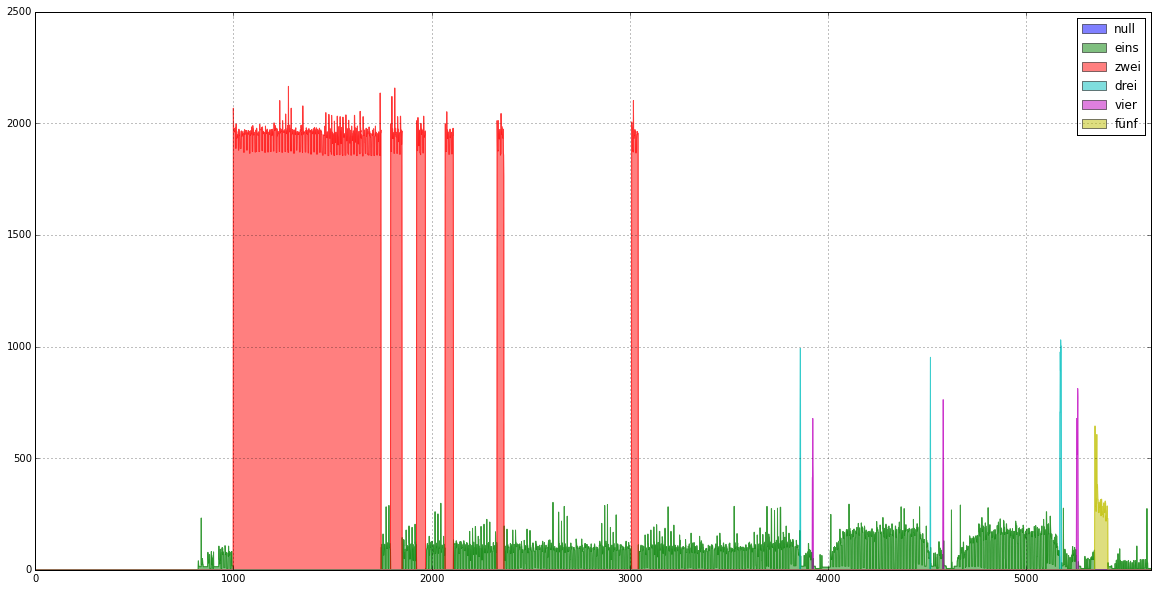
\includegraphics[height=0.8\textwidth , angle=90]{1_Grafiken/classes0.png}
	\caption[Typischer Waschgang, farbig annotiert]{Ein typischer Waschgang, je nach Klasse wird die Wirkleistung in unterschiedlichen Farben dargestellt}
\label{typWasch}
\end{figure}
